\documentclass[svgnames,tikz,serif,ragged2e]{beamer}

% Local variables for auctex, -shell-escape is needed for minted
%%% Local Variables:
%%% TeX-command-extra-options: "-shell-escape"
%%% End:

% Do hyperlinks and stuff
\usepackage{hyperref,array, tabularx}
% Add bottom bar to slides
\usepackage{beamerthemesplit}
\setbeamertemplate{navigation symbols}{}

\usepackage{relsize}
\newcommand\CC{C\nolinebreak[4]\hspace{-.05em}\raisebox{.4ex}{\relsize{-3}{\textbf{++}}}}
\newcommand\Charm{Charm\nolinebreak[4]\hspace{-.05em}\raisebox{.4ex}{\relsize{-3}{\textbf{++}}}}

\usepackage{graphicx}
\usepackage{listings}
\usepackage{textcomp}
\usepackage{inconsolata} % Use better font for code

\definecolor{ListBoxBackground}{rgb}{0.9,0.9,0.9}
\definecolor{DarkRed}{rgb}{0.7, 0.0, 0.0}
\definecolor{DarkGreen}{rgb}{0.1, 0.5, 0.0}
\definecolor{Purple}{rgb}{0.54, 0.17, 0.89}
\lstset{
  language=C++,
  aboveskip={0.1\baselineskip},
  backgroundcolor=\color{ListBoxBackground},
  basicstyle=\fontencoding{T1}\fontsize{9.8}{11}\ttfamily\bfseries,
  breakatwhitespace=true, % only break line at white space
  breaklines=true,
  captionpos=b,
  columns=fixed,
  extendedchars=false,
  frame=single, % single border around
  identifierstyle=\ttfamily,
  numbers=none,
  prebreak = \raisebox{0ex}[0ex][0ex]{\ensuremath{\hookleftarrow}},
  showspaces=false,
  showstringspaces=false,
  showtabs=false,
  tabsize=2,
  upquote=true,
  morekeywords={constexpr, noexcept},
  keywordstyle=\color{DarkGreen},
  numberstyle=\color[rgb]{0.205, 0.142, 0.73},
  commentstyle=\color{SeaGreen},
  stringstyle=\color{red}, % Below are custom emphasis words
  emph={void,short,int,float,double,TaggedTuple,Vector}, emphstyle=\color{DarkRed},
  emph={[2]charmxx,std}, emphstyle={[2]\color{Purple}},
  emph={[3]update_coordinate, apply}, emphstyle={[3]\color{blue}},
}

\newcommand{\orgspace}[0]{
  \vspace{0.3cm}
}

% Beamer theme and colours
\usetheme[width=1.8cm,hideothersubsections, hidesections]{Hannover}

\usecolortheme[named=Blue]{structure}
\setbeamercolor{frametitle}{bg=Blue!40!white}

% No header for current slide, using sidebar
\setbeamertemplate{headline}{}
\setbeamersize{sidebar width left=0pt}

% Make footer
\setbeamercolor{GitHubFooterColor}{fg=Black,bg=Blue!40!white}
\setbeamercolor{TitleFooterColor}{fg=Black,bg=Blue!30!white}
\setbeamercolor{PageNumberColor}{fg=Black,bg=Blue!20!white}
\makeatother
\setbeamertemplate{footline}
{
  \leavevmode
  \hbox{%
    \begin{beamercolorbox}[wd=.5\paperwidth,ht=2.25ex,dp=1ex,center]{GitHubFooterColor}%
      \usebeamerfont{author in head/foot}\insertshortauthor
    \end{beamercolorbox}%
    \begin{beamercolorbox}[wd=.4\paperwidth,ht=2.25ex,dp=1ex,center]{TitleFooterColor}%
      \usebeamerfont{title in head/foot}\insertshorttitle
    \end{beamercolorbox}%
    \begin{beamercolorbox}[wd=.1\paperwidth,ht=2.25ex,dp=1ex,center]{PageNumberColor}%
      \usebeamerfont{title in head/foot}
      \insertframenumber{} / \inserttotalframenumber
    \end{beamercolorbox}
  }
  \vskip0pt%
}
\makeatletter
% Done making footer

\begin{document}

% Empty square brackets means don't show in footer
\author[\href{https://github.com/sxs-collaboration/spectre}{github.com/sxs-collaboration/spectre}]
{Nils Deppe\\ Simulating eXtreme Spacetimes Collaboration}
% Empty square brackets means don't show in footer
\institute[]{Charm++ Workshop}

% Square brackets means show in footer
\date[]{April 11, 2018}
\title[A SpECTRE With a New Face] {
  \textbf{A SpECTRE With a New 'face}
}
\titlegraphic{
\includegraphics[height=.2\textheight]{sxs_logo_notext_1549px.png}
$\;\;\;\;$
\includegraphics[height=.2\textheight]{CULogo-red120px.pdf}
}



\makeatletter
% Hide the annoying info in the side bar
\setbeamertemplate{sidebar \beamer@sidebarside}{}

% Show all the subsections of the current section,
% highlighting the current subsection.
\beamer@nav@subsectionstyle{show/show/hide}
\makeatother

% What to show at the start of a section
\AtBeginSection[]
{
  \begin{frame}
    \frametitle{Table of Contents}
    \tableofcontents[currentsection,
    sectionstyle=show/show,
    subsectionstyle=show/show/hide]
  \end{frame}
}

\begin{frame}
  \titlepage{}
\end{frame}

\section{SpECTRE}


\begin{frame}
  \frametitle{SpECTRE Goals}
  Physics:
  \begin{itemize}
  \item Multi-scale, multi-physics in astrophysics
  \item Binary black holes, neutron stars
  \item Core-collapse supernovae with micro-physics
  \item Multi-disciplinary
  \end{itemize}
  HPC:\@
  \begin{itemize}
  \item Open-source, \url{https://github.com/sxs-collaboration/spectre}
  \item Efficient
  \item Exascale
  \end{itemize}
\end{frame}

\begin{frame}
  \frametitle{SpECTRE:\@ Domain Decomposition and Local Time Stepping}
  B.~Szilagyi, arXiv:~1405.3693
  \vspace{-0.4cm}
  \begin{center}
    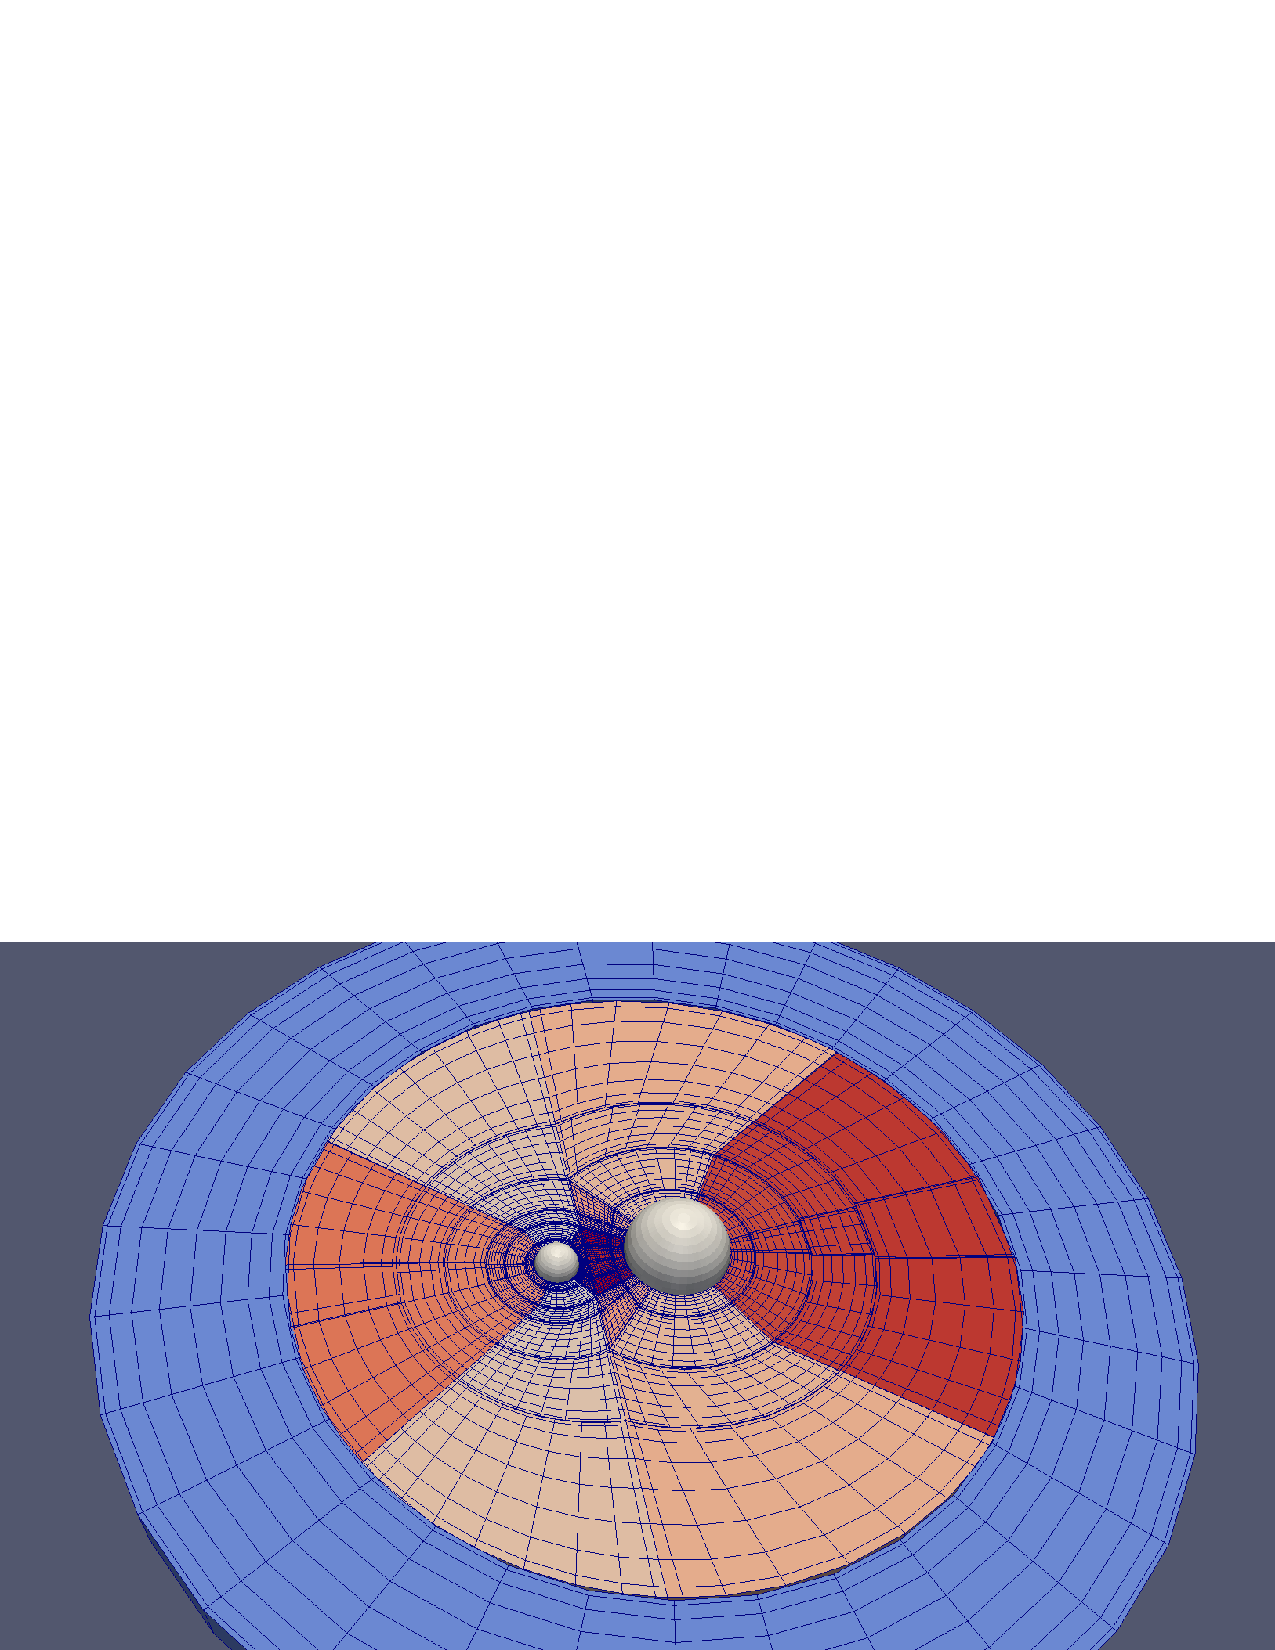
\includegraphics[height=.72\textheight]{CutSphere_SphereC0AndInterior}
  \end{center}
\end{frame}

\begin{frame}
  \frametitle{Dual Frames}
  \vspace{-0.15cm}
  \begin{center}
    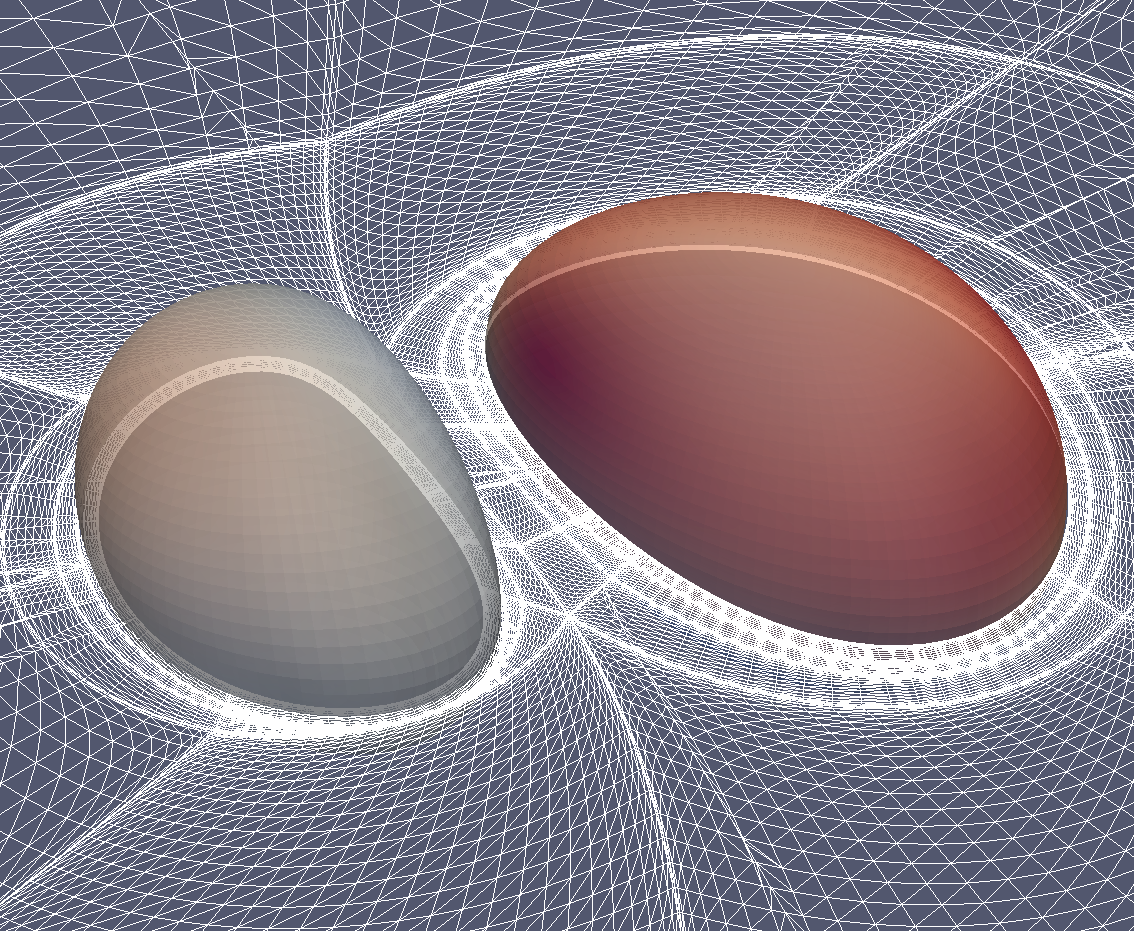
\includegraphics[height=.86\textheight]{PostUltimateGridPlusHorizons}
  \end{center}
\end{frame}

\section{The New 'face}

\begin{frame}
  \frametitle{Eliminating Charm++ Interface Files}
  Issues with interface files:
  \begin{itemize}
  \item Restrictive
  \item Error-prone (undefined behavior $\implies$ difficult bugs)
  \item Maintenance burden (users and \texttt{Charm++} devs)
  \item Can't handle modern \CC $\implies$ inefficient generated code
  \end{itemize}
  \vspace{1.0cm}

  \begin{center}
    \textit{Metaprogramming!}
  \end{center}
\end{frame}

\begin{frame}
  \frametitle{Important Features}
  We think:
  \begin{itemize}
  \item Reduce user code
  \item Really easy to use
  \item Similar to current model: familiarity $\implies$ faster adoption
  \item Error-free code generation
  \item Eliminate runtime errors
  \end{itemize}

  Any others??
\end{frame}

\begin{frame}
  \frametitle{Design Steps}
  \begin{enumerate}
  \item Invoking entry methods
  \item Creating chares
  \item Reductions
  \item Changes to code
  \end{enumerate}
\end{frame}

\begin{frame}[fragile]
  \frametitle{Invoking Entry Methods}
  Consider entry method named \texttt{MyEntryMethod}, and \texttt{Charm++} proxy
  \texttt{my\_proxy}.
  \orgspace{}

No arguments:
\begin{lstlisting}
charmxx::invoke<MyEntryMethod0>(my_proxy);
\end{lstlisting}

\orgspace{}
Passing arguments:
\begin{lstlisting}
charmxx::invoke<MyEntryMethod1>(my_proxy, arg0,
                                arg1, std::move(arg2));
\end{lstlisting}
\end{frame}

\begin{frame}[fragile]
  \frametitle{Entry Methods/Actions}
\begin{lstlisting}
struct MyEntryMethod1 {
  static void apply(const Arg0& arg0,
                    const Arg1& arg1,
                    Arg2&& arg2) noexcept {
    /* do work */
  }
};
\end{lstlisting}

  \begin{itemize}
  \item Entry methods are ``member functions''
  \item How to handle attributes?
  \item Where is chare member data?
  \end{itemize}
\end{frame}

\begin{frame}[fragile]
  \frametitle{Entry Method Attributes}
  Possible ways of controlling attributes:
  \begin{itemize}
  \item Inside entry method class
% \begin{lstlisting}
\begin{lstlisting}
struct EntryMethod0 {
  using attributes = charmxx::AttrList<
           charmxx::attr::Inline>;
  /* apply function*/
\end{lstlisting}
% \end{lstlisting}
  \item At call site
\begin{lstlisting}
charmxx::invoke<MyEntryMethod1,
         charmxx::AttrList<charmxx::attr::Inline>>(
         my_proxy, arg0, arg1, std::move(arg2));
\end{lstlisting}
  \end{itemize}
\end{frame}

\begin{frame}[fragile]
  \frametitle{Member Data}
  \begin{itemize}
  \item Chares hold a \texttt{TaggedTuple} i.e.~compile-time hash table
  \item Tags to chare as template parameter, maybe
\begin{lstlisting}
Chare<charmxx::TagList<ParticleCoordinate,
                       ParticleVelocity>>
  my_chare{start_coord, start_velocity};
\end{lstlisting}
  \item \texttt{TaggedTuple} passed to entry methods
  \end{itemize}
\end{frame}

\begin{frame}[fragile]
  \frametitle{Passing Member Data To Entry Methods}
\begin{lstlisting}
struct MyEntryMethod2 {
  template <class... Tags>
  static void apply(charmxx::TaggedTuple<Tags...>&
                      member_data,
                    const double& delta_time) noexcept {

    const auto& vel =
      charmxx::get<ParticleVelocity>(member_data);
    auto& coord =
      charmxx::get<ParticleCoordinate>(member_data);

    coord += vel * delta_time;
  }
};
\end{lstlisting}
\end{frame}

\begin{frame}[fragile]
  \frametitle{Reducing Compilation Time 1/2}
  In \texttt{MyEntryMethod2.hpp}:
\begin{lstlisting}
#include "UpdateCoordinate.hpp"

struct MyEntryMethod2 {
  template <class... Tags>
  static void apply(charmxx::TaggedTuple<Tags...>&
                      member_data,
                    const double& delta_time) noexcept {
    update_coordinate(
      charmxx::get<ParticleCoordinate>(member_data),
      charmxx::get<ParticleVelocity>(member_data),
      delta_time);
  }
};
\end{lstlisting}
\end{frame}

\begin{frame}[fragile]
  \frametitle{Reducing Compilation Time 2/2}
    In \texttt{UpdateCoordinate.hpp}:
\begin{lstlisting}
void update_coordinate(double& coord, const double& vel,
                       const double& delta_time);
void update_coordinate(Vector& coord, const Vector& vel,
                       const double& delta_time);
\end{lstlisting}
  In \texttt{UpdateCoordinate.cpp}:
\begin{lstlisting}
void update_coordinate(double& coord, const double& vel,
                       const double& delta_time) {
  coord += vel * delta_time;
}

void update_coordinate(Vector& coord, const Vector& vel,
                       const double& delta_time) {
  coord += vel * delta_time;
}
\end{lstlisting}
\end{frame}

\begin{frame}[fragile,fragile,fragile]
  \frametitle{Naming/Identifying Chares}
  Confession: I lied earlier about where tags go
\begin{lstlisting}
struct MyChareId {
  // Singleton, Array, Group, or Nodegroup
  using chare_type = charmxx::Array;
  using tags =
    charmxx::TagList<ParticleCoordinate,
                      ParticleVelocity>;
  // To put in TaggedTuple:
  using type = charmxx::compute_type<chare_type, tags>;
};
\end{lstlisting}
\end{frame}

\begin{frame}[fragile,fragile,fragile]
  \frametitle{Creating Chares}
  Create using:
\begin{lstlisting}
auto my_proxy = charmxx::create<MyChare>(start_coord,
                                         start_velocity);
auto my_proxy2 = charmxx::create<MyChare2>(
  my_proxy, start_coord, start_velocity);
\end{lstlisting}
  \begin{itemize}
  \item \texttt{create} replaces \texttt{ckNew}
  \item Chare name is also tag!
  \end{itemize}
\end{frame}

\begin{frame}[fragile]
  \frametitle{Bonus! Custom Array Indices}
  Can handle custom array indices more easily, e.g.
\begin{lstlisting}
template <size_t VolumeDim>
class ElementIndex {
 public:
  ElementIndex(const ElementId<VolumeDim>& id) noexcept;

 private:
  std::array<SegmentIndex, VolumeDim> segments_;
};
\end{lstlisting}
  \texttt{ElementId} indexes block, $x$, $y$, and $z$ in domain
\end{frame}

\begin{frame}[noframenumbering]
  \frametitle{Design Steps}
  \begin{enumerate}
  \item Invoking entry methods
  \item Creating chares
  \item \textbf{Reductions}
  \end{enumerate}
\end{frame}

\begin{frame}[fragile,fragile]
  \frametitle{Reductions}
  \begin{itemize}
  \item<1-> Reductions become quite straight forward:
\begin{lstlisting}
charmxx::contribute_to_reduction<
      ProcessReducedProductOfDoublesEntryMethod>(
  receiver_proxy, array_proxy,
  charmxx::Reduction::product_double,
  my_send_double);
\end{lstlisting}
  \item<2-> Reducing custom data also simpler
  \item<2-> Supply generic data structure for custom reductions
\begin{lstlisting}
charmxx::ReductionData<int,
                       double,
                       std::vector<double>>;
\end{lstlisting}
  \end{itemize}
\end{frame}

\begin{frame}[fragile]
  \frametitle{Custom Reductions}
  Function to reduce custom data structure:
\begin{lstlisting}
charmxx::ReductionMsg* reduce_reduction_data(
      const int number_of_messages,
      charmxx::ReductionMsg** const msgs) noexcept {
  /* custom reduction function*/
}
\end{lstlisting}

  \pause
  Inside an entry method:
\begin{lstlisting}
charmxx::contribute_to_reduction<
      &reduce_reduction_data,
      ProcessCustomReductionEntryMethod>(
  receiver_proxy, array_proxy,
  charmxx::ReductionData<int,
                         std::unordered_map<std::string,
                                            int>,
                         std::vector<int>>{
  10, my_send_map,
  std::vector<int>{array_index, 10, -8}});
\end{lstlisting}
\end{frame}

\begin{frame}
  \frametitle{Summary}
  \begin{itemize}
  \item \texttt{Charm++} can be replaced with basic metaprogramming
  \item Users do not need to know metaprogramming
  \item Large number of errors are eliminated
  \item Most remaining errors are compile time
    \item Integrate into \texttt{Charm++} v7?
  \end{itemize}
\end{frame}

\end{document}